\documentclass{if-beamer}
\usepackage{xcolor}
\setbeamertemplate{footline}[frame number]
\usepackage{multicol}
%
% Choose how your presentation looks.
%
% For more themes, color themes and font themes, see:
% http://deic.uab.es/~iblanes/beamer_gallery/index_by_theme.html
%
\mode<presentation>
{
  \usetheme{default}      % or try Darmstadt, Madrid, Warsaw, ...
  \usecolortheme{default} % or try albatross, beaver, crane, ...
  \usefonttheme{default}  % or try serif, structurebold, ...
  \setbeamertemplate{navigation symbols}{}
  \setbeamertemplate{caption}[numbered]
} 

\usepackage{tikz}
\usetikzlibrary{shapes}
\usepackage{tcolorbox}
\usepackage[english]{babel}
\usepackage[utf8]{inputenc}
\usepackage[T1]{fontenc}
\usepackage{mathtools}
\newcommand{\defeq}{\vcentcolon=}
\newcommand{\eqdef}{=\vcentcolon}
\newcommand{\norm}[2]{\left\lVert#1\right\rVert_{#2}}
\DeclarePairedDelimiter{\ceil}{\lceil}{\rceil}
\newcommand*\circled[1]{\tikz[baseline=(char.base)]{
            \node[shape=circle,draw,inner sep=0.2pt] (char) {#1};}}
\newcommand\STAR{\raisebox{-.7em}{\tikz{\node[draw,star,star point height=.7em,minimum size=1em]{};} }}


\title[Neural Networks in Approximation]{Mathematical Techniques in the Approximation Theory that are Rooted in Neural Networks - Hieber's Theorem}
\author{Suh, Ko, Huo}
\institute{Georgia Tech}
\date{Summer of 2020}
\graphicspath{{figures/}}

\begin{document}

\begin{frame}
  \titlepage
\end{frame}

\begin{frame}
    \frametitle{Outline}
    \begin{multicols}{2}
        \tableofcontents
    \end{multicols}
\end{frame}

\section{Preliminaries}
\subsection{Mathematical Problem}
\begin{frame}{Mathematical Problem}
\begin{itemize}
    \item Given a function $f \in \mathcal{C}$ where $\mathcal{C}$ is some class of functions, how many weights, nodes, and layers does one need to approximate $f$ with certain accuracy in some predefined metric?
\end{itemize}
\end{frame}

\subsection{A Neural Network Class to be considered}
\begin{frame}{A Neural Network Class to be considered}
    We first introduce the formal mathematical representation of the FNN model as follows: 
    \begin{itemize}
        \item The network architecture $(L,\textbf{p})$ consists of a positive integer $L$ called the number of hidden layers and a width vector $\textbf{p}=(p_0,\dots,p_{L+1})$. 
        
        \item $\sigma$ denotes a ReLU activation function, where it is defined as $\sigma(x)=\mbox{max}(x,0)$. 
        
        \item For $\textbf{v}=(v_{1},\dots,v_{r})\in\mathbb{R}^{r}$, define a shifted activation function $\sigma_{\textbf{v}}:\mathbb{R}^{r}\rightarrow{\mathbb{R}^{r}}$. 
        \begin{equation*}
            \sigma_{\textbf{v}}
            \begin{pmatrix} y_{1} \\ \vdots \\ y_{r}\end{pmatrix}
            =
            \begin{pmatrix} \sigma( y_{1} - v_{1} ) \\ \vdots \\ \sigma( y_{r} - v_{r} ) \end{pmatrix}.
        \end{equation*}
    \end{itemize}
\end{frame}

\begin{frame}{A Neural Network Class to be considered}
    Neural network with network architecture $(L,\textbf{p})$ is any function of form
    \begin{eqnarray}\label{eq:eq1} 
            f:\mathbb{R}^{P_0}\rightarrow{\mathbb{R}^{P_{L+1}}}, f(x)=W_L\sigma_{V_{L}}W_{L-1}\sigma_{V_{L-1}}\dots W_1\sigma_{V_{1}}W_0x,
    \end{eqnarray}
    where $W_i$ is a $p_{i+1}\times p_{i}$ weight matrix and $v_i \in \mathbb{R}^{p_i}$ is a shift vector. 

    \begin{figure}[htbp]
        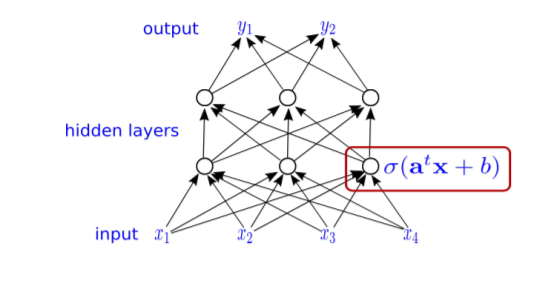
\includegraphics[width=0.75\textwidth]{Network_architecture.png}
        \caption{ Representation as a direct graph of a network with $2$ hidden layers $L=2$ and width vector $\textbf{p}=(4,3,3,2)$.  }
        \label{fig:figure1}
    \end{figure}
\end{frame}

\begin{frame}{A Neural Network Class to be considered}
    \begin{itemize}
        \item All parameter values in the network are bounded by one:
        \begin{eqnarray*}
            \mathcal{F}(L,\textbf{p}):=\big\{ f \mbox{ of the form } \eqref{eq:eq1} : \max_{j=0,\dots,L}\|W_j\|_{\infty} \vee |v_j|_{\infty} \leq 1 \big\},
        \end{eqnarray*}
        where $\|W_j\|_{\infty}$ denotes the maximum entry norm of $W_j$.
        
        \item There are only a few non-zero/active network parameters: 
        \begin{eqnarray*}
            \sum^{L}_{j=0}\|W_j\|_{0} + |v_j|_{0} \leq s.
        \end{eqnarray*}
        where $\|W_j\|_{0}$ denotes the number of non-zero entries of $W_j$.

        \item Combining all the imposed assumptions, we are going to consider a neural network class whose architecture is constructed as follows: 
        \begin{equation*}
            \mathcal{F}(L,\textbf{p},s,F)
            :=\bigg\{ f(x) \in \mathcal{F}(L,\textbf{p}) : \sum^{L}_{j=0}\|W_j\|_{0}+
            |v_j|_{0} \leq s, \left\| f \right\|_{\infty} \leq F \bigg\}.
        \end{equation*}
    \end{itemize}
\end{frame}

\subsection{Assumption on Regression function}
\begin{frame}{Assumption on Regression function}
In this page, we introduce a multi-index notation which will be frequently used in following slides. For $r$-dimensional vectors, $a\in[0,1]^{r}$, $x=(x_{1},\dots,x_{r})$ and $\boldsymbol{\alpha}=(\alpha_{1},\dots,\alpha_{r})$.
\begin{itemize}
    \item 
    \begin{equation*}
        x^{\boldsymbol{\alpha}} := x_{1}^{\alpha_{1}}\cdots x_{r}^{\alpha_{r}}.
    \end{equation*}
    
    \item 
    \begin{equation*}
        \left| (x-a)^{\boldsymbol{\alpha}} \right| := \prod_{i=1}^{r} \left| x_{i} - a_{i} \right|^{\alpha_{i}}.
    \end{equation*}
    
    \item 
    \begin{equation*}
        |\boldsymbol{\alpha}| := |\alpha_{1}|+\cdots+|\alpha_{r}|.
    \end{equation*}
    
    \item 
    \begin{equation*}
        \partial^{\boldsymbol{\alpha}}{f} := 
        \frac{\partial^{\alpha}}{\partial^{\alpha_{1}}\cdots\partial^{\alpha_{r}}}f.
    \end{equation*}
\end{itemize}
\end{frame}


\begin{frame}{Assumption on Regression function}
\begin{itemize}
    \item H\"older class with $\beta$-smoothness index is one of the most commonly studied function classes in literature.
    \item For $\beta=n+\sigma$ where $n \in \mathbb{N}_{0}$ and $\sigma \in (0,1]$, a function has h\"older smoothness index $\beta$ if all partial derivatives up to order $n$ exist and are bounded and the partial derivatives of order $n$ are $\sigma$ h\"older.
    \item The ball of $\beta$-h\"older functions with radius $K$ is then defined as 
        \begin{eqnarray*}
            \mathcal{C}_{r}^{\beta}(D,K) = &\bigg\{ f : D\subset \mathbb{R}^{r} \rightarrow{\mathbb{R}} : 
            \sum_{\boldsymbol{\alpha}:|\boldsymbol{\alpha}|\leq n} \|\partial^{\boldsymbol{\alpha}}{f}\|_{\infty} + \\ &\sum_{\boldsymbol{\alpha}:|\boldsymbol{\alpha}|=n} \sup_{\substack{\boldsymbol{x}, \boldsymbol{y} \in D \\ \boldsymbol{x} \ne \boldsymbol{y}}} \frac{|\partial^{\boldsymbol{\alpha}}f(\boldsymbol{x}) - \partial^{\boldsymbol{\alpha}}f(\boldsymbol{y})|}{|\boldsymbol{x}-\boldsymbol{y}|_{\infty}^{\sigma}} \leq K \bigg\}. \nonumber
        \end{eqnarray*}
    \item In Hieber (2020), $D=[0,1]^{r}$. In Petersen and Voigtlaender (2018), $D=[-\frac{1}{2},\frac{1}{2}]^{r}$ where $r$ is an input dimension.
\end{itemize}
\end{frame}

\section{Theorem Statement}
\begin{frame}{Theorem 5 of Hieber 2020}
\begin{tcolorbox}
    For any function $f\in\mathcal{C}_{r}^{\beta}([0,1]^{r},K)$ and any integers $m\geq 1$ and $N\geq(\beta+1)^{r} \vee (K+1)e^{r}$, there exists a network 
    \begin{equation*}
        \Tilde{f}\in\mathcal{F}\big(L,(r,6(r+\ceil[\big]{\beta})N,\dots,6(r+\ceil[\big]{\beta})N,1),s,\infty\big)
    \end{equation*}
    with depth
    \begin{equation*}
        L=8+(m+5)\big(1+\ceil[\big]{\log_{2}(r\vee\beta)}\big)
    \end{equation*}
    and the number of parameters 
    \begin{equation*}
        s\leq 141(r+\beta+1)^{3+r}N(m+6),
    \end{equation*}
    such that
    \begin{equation*}
        \left\|\Tilde{f}-f\right\|_{L^\infty[0,1]^{r}}\leq (2K+1)(1+r^{2}+\beta^{2})6^{r}N2^{-m}+K3^{\beta}N^{-\frac{\beta}{r}}.
    \end{equation*}
\end{tcolorbox}
\end{frame}

\section{Key Ideas}
\subsection{Key Ideas for proof of Theorem}
\begin{frame}{Key Ideas for proof of Theorem}
    Key ideas for approximating functions in $\mathcal{C}_{r}^{\beta}(D,K)$ with Neural Network are mainly two folded:
    \begin{itemize}
        \item Local Taylor Approximation : We split the input space into small hyper-cubes and construct a network that approximates a local Taylor expansion on each of these hyper-cubes.
        \item Approximation of multiplication operator : We need to build networks that for given input $(x,y)$ approximately compute the product $xy$. 
    \end{itemize}
\end{frame}

\subsection{Local Taylor Approximation}
\begin{frame}{Local Taylor Approximation?}
    \begin{itemize}
      \item Discretize the input space $[0,1]^{r}$ with a set of points     $D(M):=\{X_{\ell}=(\ell_{j}/M)_{j=1,2,\dots,r},\ell=(\ell_{1},\ell_{2},\dots,\ell_{r}) \in\{0,1,2,\dots,M\}^{r}\}$. The cardinality of this set is $(M+1)^{r}$.
      \item Think of Taylor expansion of $f(x)$ at one of the grid points, $x_{\ell}\in D(M)$, with up to degree $n$, which can be written as 
    \begin{equation*}
        P_{x_{\ell}}^{\beta}f(x):=\sum_{\alpha:|\alpha|\leq n}(\partial^{\alpha}f)(x_{\ell})\frac{(x-x_{\ell})^{\alpha}}{\alpha!}.
    \end{equation*}
      \item For an arbitrary input $x\in[0,1]^{r}$, Local Taylor approximation of $f\in \mathcal{C}_{r}^{\beta}([0,1]^{r},K)$ can be written as follows:
    \begin{equation*}
        P^{\beta}f(x):=\sum_{x_{\ell}\in D(M)}P_{x_{\ell}}^{\beta}f(x)\prod_{j=1}^{r}\bigg( 1- M|x_{j}-x_{j}^{\ell}| \bigg)_{+},
    \end{equation*}
    where $x=\{x_{1},x_{2},\dots,x_{r}\}$.
    \end{itemize}
\end{frame}

\begin{frame}{Local Taylor Approximation?}
    \begin{itemize}
        \item $\forall x \in [0,1]^{r}$, Local Taylor Approximation of $f(x)$ is written as linear combination of $2^{r}$ terms of $P^{\beta}_{x_{\ell}}f(x)$, for which $x_{\ell}\in D(M)$ such that $\left\| x - x_{\ell} \right\|_{\infty}\leq \frac{1}{M}$.
    \end{itemize}
    \begin{figure}[htbp]
        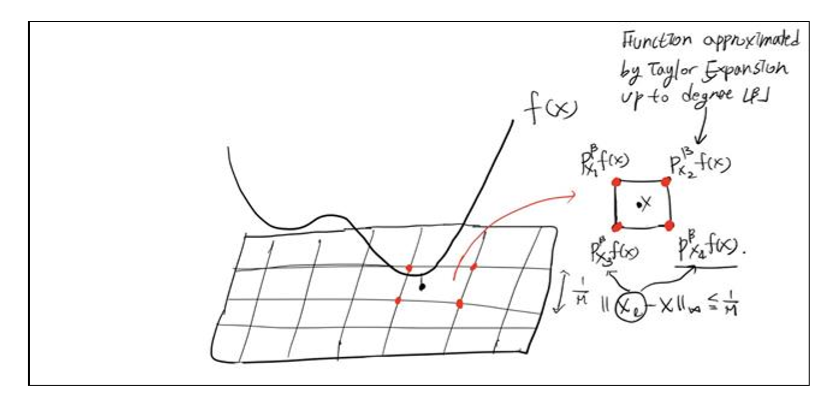
\includegraphics[width=0.8\textwidth]{LTA.png}
        \caption{ Visualization of intuition on Local Taylor Approximation when $r=2$.}
        \label{fig:figure1}
    \end{figure}
\end{frame}

\addtocontents{toc}{\newpage}           % Splits manually the ToC into 2 columns
\section{First Step}
\begin{frame}{First Step}
    \begin{itemize}
    \item Neural Network $\Tilde{f}$ is not directly used to approximate $f\in\mathcal{C}^{\beta}_{r}([0,1]^{r},K)$, instead it is used to approximate the approximated $f$ through local Taylor expansion, where we denote it as $P^{\beta}f(X)$.
    \item For $X\in[0,1]^{r}$, the closeness between functions is measured in a $L^{\infty}$ sense. Approximation error can be decomposed with the help of triangular inequality as follows:
    \begin{eqnarray*}
        \scriptsize
        \left\| \Tilde{f} - f \right\|_{L^\infty[0,1]^{r}}
        \leq \underbrace{\left\| P^{\beta}f(X) - f(X) \right\|_{L^\infty[0,1]^{r}}}_{\circled{1}} + 
        \underbrace{\left\| \Tilde{f} - P^{\beta}f(X) \right\|_{L^\infty[0,1]^{r}}}_{\circled{2}} .
    \end{eqnarray*}
    
    \item Controlling $\circled{2}$ will be the main focus, whereas a term $\circled{1}$ can be easily controlled trough the definition of H\"older class. 
    \end{itemize}
\end{frame}

\begin{frame}{Control on $\circled{1}$}
    Observe $f(x)$ can be written as follows by Multivariate Taylor's Theorem: for any $\xi \in [0,1]$ and any $a \in [0,1]^{r}$,
    \begin{equation*}
        \tiny
        f(x)=\sum_{\alpha:|\alpha|\leq n-1}\partial^{\alpha}f(a)\frac{(x-a)^{\alpha}}{\alpha!}+
        \sum_{\alpha:|\alpha|=n}\partial^{\alpha}f(a+\xi(x-a))\frac{(x-a)^{\alpha}}{\alpha!}.
     \end{equation*}
    So for $f\in\mathcal{C}^{\beta}_{r}([0,1]^{r},K)$ ,
    \begin{eqnarray*}
        |f(x)-P^{\beta}_{a}f(x)| &=& \sum_{\alpha:|\alpha|=n}\left|\partial^{\alpha}f(a+\xi(x-a))-\partial^{\alpha}f(a)\right|\frac{\left|(x-a)^{\alpha}\right|}{\alpha!} \\
        &\leq& K|x-a|_{\infty}^{\beta}.
    \end{eqnarray*}
\end{frame}

\begin{frame}{Control on $\circled{1}$}
    It is interesting to observe a following fact
    \begin{equation*}
        \sum_{x_{\ell}\in D(M)}\prod_{j=1}^{r}\bigg( 1- M|x_{j}-x_{j}^{\ell}| \bigg)_{+}
        =\prod_{j=1}^{r}\sum_{\ell=1}^{M}\bigg( 1- M\left|x_{j}-\frac{\ell}{M}\right| \bigg)_{+}=1.
    \end{equation*}
    By using this relation, we can see
    \begin{eqnarray*}
        \tiny
        &&\left\| P^{\beta}(x) - f(x) \right\|_{L^\infty[0,1]^{r}} \\ 
        &&=\left| \sum_{x_{\ell}\in D(M)}\bigg(\underbrace{P_{x_{\ell}}^{\beta}f(x)-f(x)}_{\leq K|x-x_{\ell}|_{\infty}^{\beta}}\bigg)\prod_{j=1}^{r}\bigg( 1- M|x_{j}-x_{j}^{\ell}| \bigg)_{+} \right|_{\infty} \\
        &&\leq KM^{-\beta}.
    \end{eqnarray*}
\end{frame}

\section{Second Step}
\begin{frame}{Second Step}
    In order to control the term $\circled{2}$, of course, we first need to build a Neural network which can approximate $P^{\beta}(X)$. This step is involved with several sub-steps:
    \begin{enumerate}
        \item For all $x_{\ell}\in D(M)$ and for an arbitrary input $x\in [0,1]^{r}$, we need to build a Neural Network which can approximate $P^{\beta}_{x_\ell}(x)$. 
        Constructed Neural Network has output in $\mathbb{R}^{(M+1)^{r}}$.
        \item For all $x_{\ell}\in D(M)$ and for an arbitrary input $x\in [0,1]^{r}$, we need to build a Neural Network which can approximate $\prod_{j=1}^{r}\bigg( \frac{1}{M}- |x_{j}-x_{j}^{\ell}| \bigg)_{+}$. 
        Constructed Neural Network has output in $\mathbb{R}^{(M+1)^{r}}$ as well.
    \end{enumerate}
\end{frame}

\subsection{Involved Tools for approximating $P_{x_{\ell}}^{\beta}f(x)$}
\begin{frame}{Involved Tools for approximating $P_{x_{\ell}}^{\beta}f(x)$}
    Through a $r$-dimensional Binomial theorem, we can write $P^{\beta}_{x_{\ell}}(x)$ as linear combination of monomials: 
    \begin{equation*}
        P_{x_{\ell}}^{\beta}f(x):=\sum_{\alpha:|\alpha|\leq n}(\partial^{\alpha}f)(x_{\ell})\frac{(x-x_{\ell})^{\alpha}}{\alpha!}
        = \sum_{\gamma:|\gamma|\leq n} C_{\gamma}x^{\gamma}.
    \end{equation*}
    In order to construct a neural network which can approximate $P_{x_{\ell}}^{\beta}f(x)$ for a $x_{\ell}$, we need following tools:
    \begin{enumerate}
        \item Multiplication operator $Mult_{m}(x,y)$ which can approximate the product of two input data $x,y$.
        \item Product operator $Mult_{m}^{r}(x_{1},\dots,x_{r})$ which can approximate $\Pi_{j=1}^{r}x_{j}$ for an input data $x\in[0,1]^{r}$.
        \item Monomial operator $Mon_{m,\gamma}^{r}(x_{1},\dots,x_{r})$ which can approximate all monomials with up to degree $|\gamma|\leq n$.
    \end{enumerate}
\end{frame}

\subsection{Lemma A.1.}
\begin{frame}{Lemma A.1.}
    In order to construct a neural network which can compute the product of two input data, we first need to have a ReLU neural network which can approximate $x(1-x)$ for an $x\in\mathbb{R}$.
    \begin{tcolorbox}
    \textbf{(Lemma A.1.)}
    Let $T^{k}:[0,2^{2-2k}]\rightarrow{[0,2^{k}}]$,
    \begin{equation*}
        T^{k}(x) := T_{+}(x) - T_{-}^{k}(x) = (x/2)_{+} - (x-2^{1-2k})_{+},
    \end{equation*}
    and $R^{k}:[0,1]\rightarrow{[0,2^{-2k}]}$,
    \begin{equation*}
        R^{k}(x) := T^{k}\circ T^{k-1} \circ, \dots, T^{1}.
    \end{equation*}
    Then, for any positive integer $m$,
    \begin{equation*}
        \left| x(1-x) - \sum_{k=1}^{m} R^{k}(x) \right| \leq 2^{-m}.
    \end{equation*}
    
    \end{tcolorbox}
    
    Detailed proof using induction can be found in the paper. 
\end{frame}

\begin{frame}{Visual Illustration of Lemma A.1. }

    \begin{figure}[htbp]
        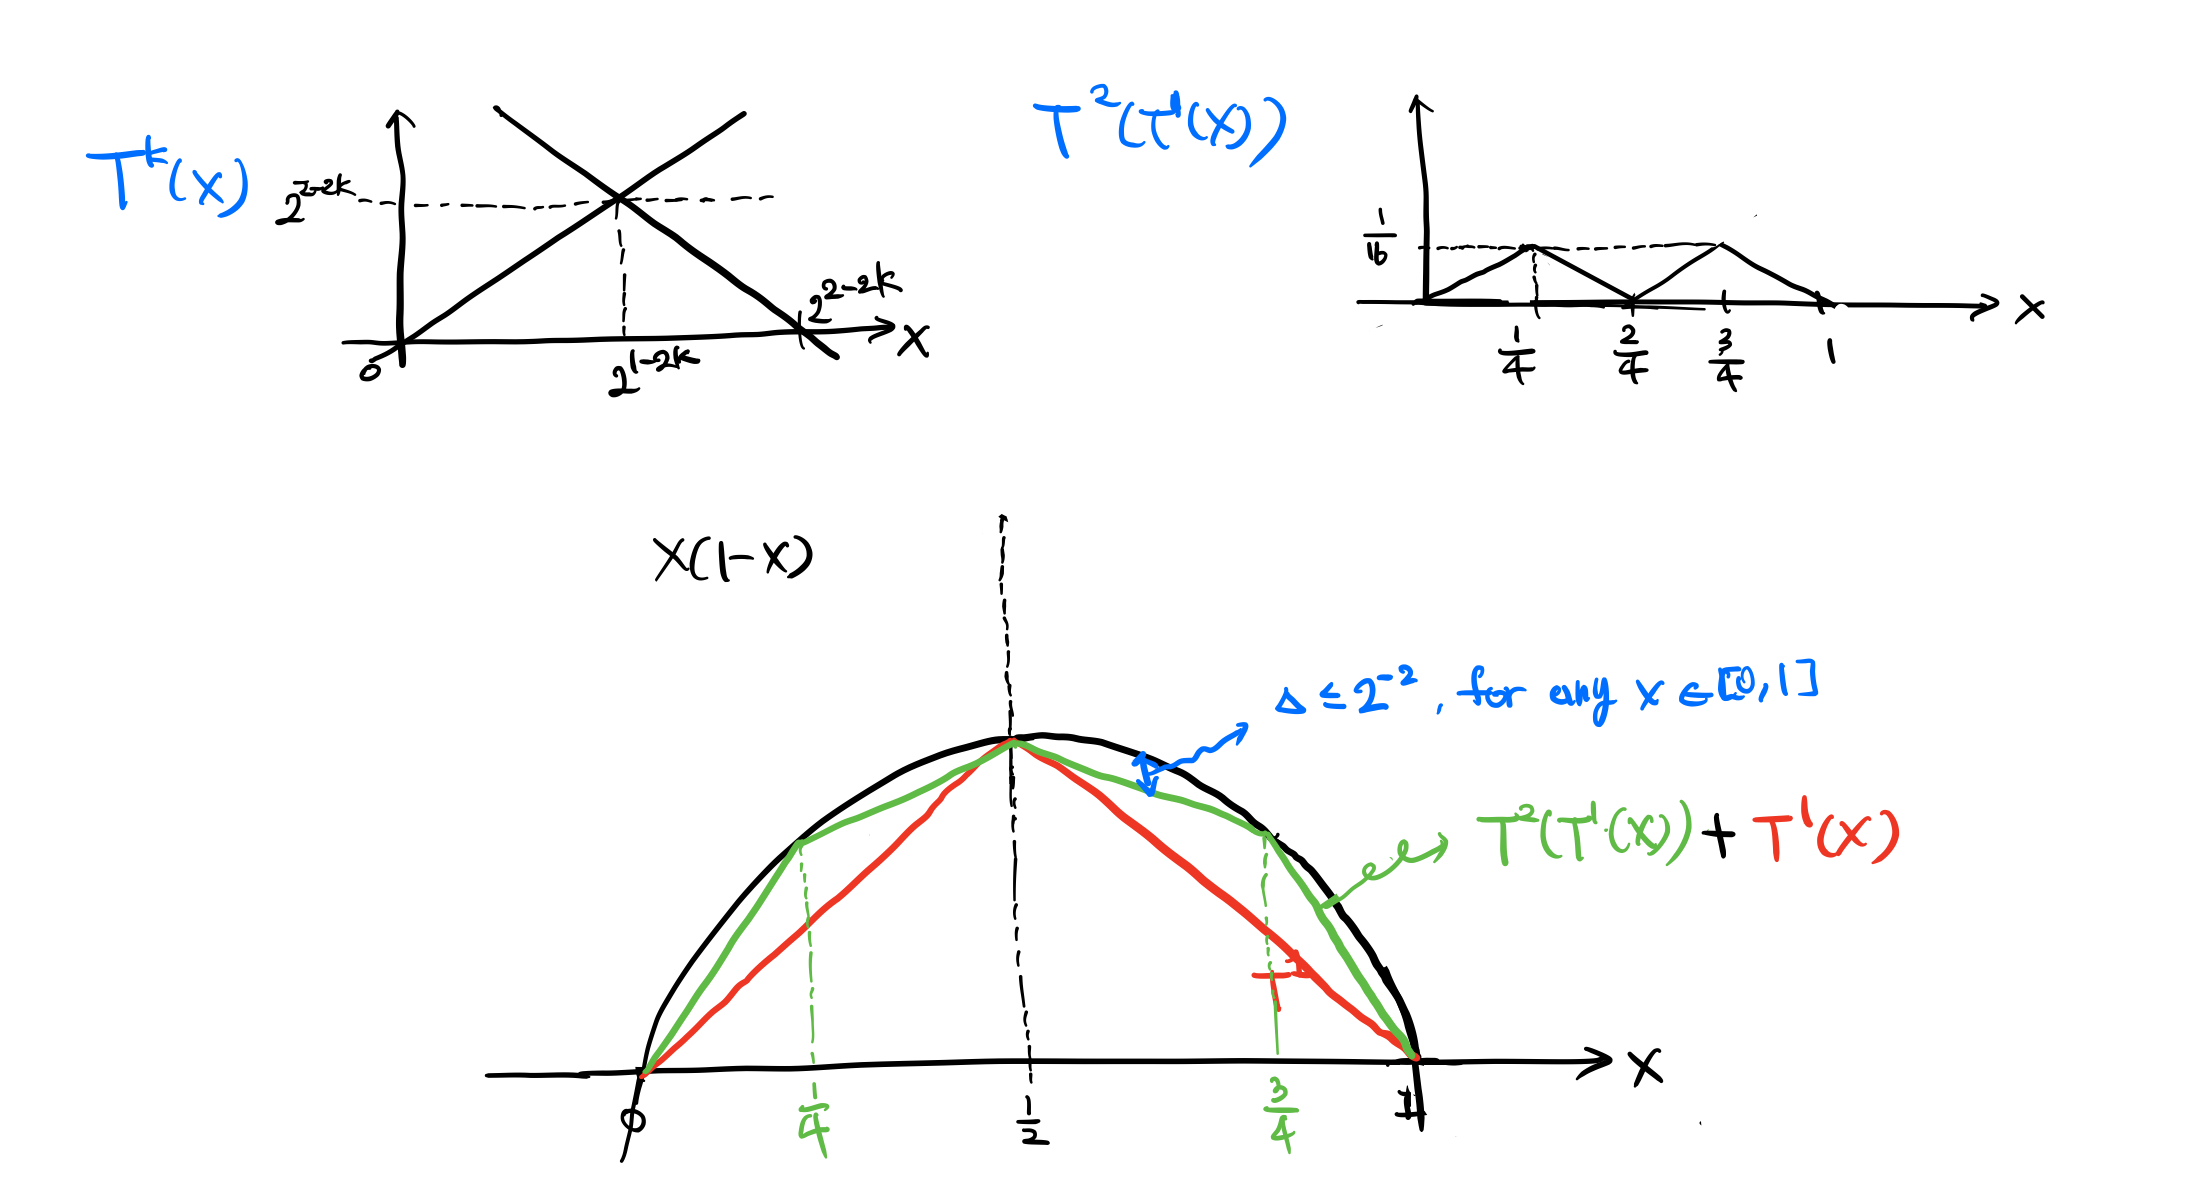
\includegraphics[width=1\textwidth]{approx.png}
        \caption{ Intuition behind Lemma A.1. can be easily captured by visualization. The Lemma can be proved rigorously via proof by induction on $m$. }
        \label{fig:figure2}
    \end{figure}

\end{frame}

\subsection{Realization of $Mult_{m}(x,y)$}
\begin{frame}{Realization of $Mult_{m}(x,y)$}
    For given input $x,y$, we construct a network which returns 
    approximately $xy$.
    
    \begin{tcolorbox}
    \textbf{(Lemma A.2.)}
    For any positive integer $m$, there exists a network $Mult_m \in \mathcal{F}(m+4,(2,6,6,\dots,6,1))$, such that $Mult_m(x,y)\in[0,1]$,
    \begin{equation*}
        \left|Mult_m(x,y)-xy\right|\leq 2^{-m}, \quad \forall x, y \in [0,1],
    \end{equation*}
    and $Mult_m(x,0)=Mult_m(0,y)=0$.
    \end{tcolorbox}
    \begin{enumerate}
        \item Let $g(x)=x(1-x)$ and use a following polarization identity : 
        \begin{equation*}
            xy = \underbrace{\bigg( g\bigg( \frac{x-y+1}{2} \bigg) + \frac{x+y}{2} \bigg)}_{\circled{1}} - \underbrace{\bigg( g\bigg( \frac{x+y}{2} \bigg) + \frac{1}{4} \bigg)}_{\circled{2}}
        \end{equation*}
        \item Our goal is to construct two neural networks which can approximate $\circled{1}$ and $\circled{2}$. 
    \end{enumerate}

\end{frame}

\begin{frame}{Realization of $Mult_{m}(x,y)$}
    We can show that there is a network $N_m$ with $m$ hidden layers and width vector $(3,3,3,\dots,3,1)$ that computes the function $(T_{+}(u),T_{-}^{1}(u),h(u))\rightarrow{\sum_{k=1}^{m+1}R^{k}(u)+h(u)}$.
    \begin{figure}[htbp]
        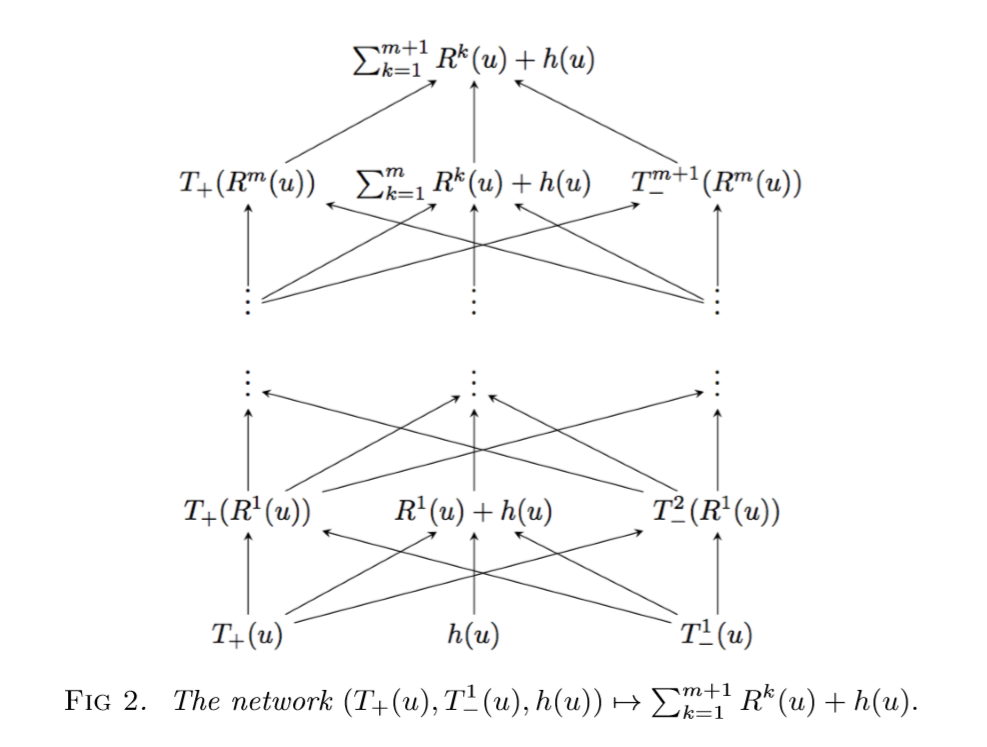
\includegraphics[width=0.7\textwidth]{approx_prod.png}
        \label{fig:figure3}
    \end{figure}
\end{frame}

\begin{frame}{Realization of $Mult_{m}(x,y)$}
    \begin{enumerate}
        \item Note that all weight parameters' absolute values are bounded by $1$ in network $N_m$.
        \item Set $u=\frac{x-y+1}{2}$, $h(u)=\frac{x+y}{2}$ and apply $N_m$ to approximate $\circled{1}$. Set $u=\frac{x+y}{2}$, $h(u)=\frac{1}{4}$ and apply $N_m$ to approximate $\circled{2}$. 
        \item Concatenate two constructed networks in parallel, then we have a network with $m+1$ hidden layers and width vector $(2,6,6,\dots,6,2)$ that computes:
    \end{enumerate}
     \begin{equation*}
        (x,y) \rightarrow{\bigg(\underbrace{\sum_{k=1}^{m+1}R^{(k)}\bigg(\frac{x-y+1}{2}\bigg)+\frac{x+y}{2}}_{=a},\underbrace{\sum_{k=1}^{m+1}R^{(k)}\bigg(\frac{x+y}{2}\bigg)+\frac{1}{4}\bigg)}_{=b}}
    \end{equation*}
\end{frame}

\begin{frame}{Realization of $Mult_{m}(x,y)$}
To ensure the final output to be in $[0,1]$, we apply to the $a, b$ the two hidden layer network 
\begin{equation*}
    (a,b)\rightarrow{(1-(1-(a-b))_{+})_{+}}=(a-b)_{+}\wedge 1.
\end{equation*}

Error bound for approximating $xy$ can be derived as follows:
\begin{eqnarray*}
    \left|Mult_{m}(x,y)-xy\right| &&\leq \left| \sum_{k=1}^{m+1}R^{(k)}\bigg(\frac{x-y+1}{2}\bigg) - g\bigg( \frac{x-y+1}{2} \bigg) \right| \\
    && + \left| \sum_{k=1}^{m+1}R^{(k)}\bigg(\frac{x+y}{2}\bigg) - g\bigg( \frac{x+y}{2} \bigg) \right| \\
    && \leq 2^{-m-1}+2^{-m-1} = 2^{-m}.
\end{eqnarray*}
\end{frame}

\subsection{Realization of $Mult_{m}^{r}(x_{1},\dots,x_{r})$}
\begin{frame}{Realization of $Mult_{m}^{r}(x_{1},\dots,x_{r})$}
Next goal is to construct a product operator which returns approximately $\prod_{i=1}^{r}x_{i}$ for $\textbf{x}\in[0,1]^{r}$.

\begin{tcolorbox}
    \textbf{(Lemma A.3.)}
    For any positive integer $m$, there exists a network 
    \begin{equation*}
        Mult_m^{r} \in \mathcal{F}( (m+5)\ceil{log_{2}r},(r,6r,6r,\dots,6r,1))
    \end{equation*}
    such that $Mult_m^{r}\in[0,1]$ and
    \begin{equation*}
        \left| Mult_m^{r}(X) - \prod_{i=1}^{r}x_{i} \right| \leq r^{2}2^{-m},
        \quad \forall \textbf{x}=(x_{1},x_{2},\dots,x_{r})\in[0,1]^{r}.
    \end{equation*}
    Moreover, $Mult_m^{r}(x)=0$ if one of the components of $x$ is zero.
\end{tcolorbox}

\end{frame}

\begin{frame}{Realization of $Mult_{m}^{r}(x_{1},\dots,x_{r})$}

\begin{enumerate}
    \item For $q=\ceil{log_{2}r}$, construct a first hidden layer as follows:
    \begin{equation*}
        (x_{1},\dots,x_{r})\rightarrow{\big(x_{1},\dots,x_{r},\underbrace{1,\dots,1}_{=2^{q}-r} \big)}.
    \end{equation*}
    \item Apply the network $Mult_m$ in Lemma A.2. to the pairs $(x_1,x_2)$,$(x_3,x_4)$,\dots,$(1,1)$ in order to compute $(Mult_m(x_{1},x_{2}),\dots,Mult_m(1,1))\in\mathbb{R}^{2^{q-1}}$.
    \item Repeat Step 2. until there is only one entry left.
    \item The resulting network is called $Mult_{m}^{r}$ and has $q(m+5)$ hidden layers and all parameters bounded by one.
\end{enumerate}

\end{frame}

\begin{frame}{Error bound on $Mult_{m}^{r}(x_{1},\dots,x_{r})$}
 For $q=1$, the bound holds trivially by Lemma A.2. \\
 Assume that when $q=k-1$, a following bound holds: 
    \begin{equation*}
        \left| Mult_m^{r}(X) - \prod_{i=1}^{r}x_{i} \right| \leq 3^{k-2}2^{-m}.
    \end{equation*}
 We set $a,b,c,d \in [0,1]$ as follows:
 \begin{enumerate}
     \item a : Output of network 1, $Mult_m^{r}(x)$, when $q=k-1$.
     \item b : Output of network 2, $Mult_m^{r}(x)$, when $q=k-1$.
     \item c : The true value of product network 1 should have.
     \item d : The true value of product network 2 should have.
 \end{enumerate}   
 
 \STAR We want to check $\left| Mult_{m}(a,b) - cd \right|\leq 3^{k-1}2^{-m}\leq r^{2}2^{-m}$.
 
\end{frame}


\begin{frame}{Error bound on $Mult_{m}^{r}(x_{1},\dots,x_{r})$}

\STAR We want to check $\left| Mult_{m}(a,b) - cd \right|\leq 3^{k-1}2^{-m}\leq r^{2}2^{-m}$.

\begin{eqnarray*}
    \left| Mult_{m}(a,b) - cd \right| &=& 
    \left| Mult_{m}(a,b) - ab + ab - cd \right| \\
    &\leq& \left| Mult_{m}(a,b) - ab \right| +\left| ab - cd \right| \\
    &=& 2^{-m} + \left| ab-bc+bc-cd \right| \\
    &\leq& 2^{-m} + \left| b \right| \left| a-c \right| + \left| c \right| \left|b-d \right|\\
    &\leq& 2^{-m} + 3^{k-2}2^{-m} + 3^{k-2}2^{-m}\\
    &\leq& 3^{k-1}2^{-m} \leq r^{2}2^{-m},
\end{eqnarray*}
where in the last inequality, we use the fact
$k=q$ and $(q-1)\log(3)<2(q-1)<2\log_{2}r=\log_{2}r^{2}$.

\end{frame}

\subsection{Realization of $Mon_{m,\gamma}^{r}(x_{1},\dots,x_{r})$}
\begin{frame}{Realization of $Mon_{m,\gamma}^{r}(x_{1},\dots,x_{r})$}
\begin{enumerate}
    \item Using the network operator $Mult_m^{r}$, we are now ready to construct a network which can approximate all monomials of input data $x\in[0,1]^{r}$ with degree up to $|\alpha| \leq n$. 
    \item Here we use a multi-index notation and $C_{r,\gamma}$ denotes total number of monomials with degree up to $|\alpha| \leq n$. 
\end{enumerate}
\begin{tcolorbox}
    \textbf{(Lemma A.4.)}
    For $\gamma>0$ and any positive integer $m$, there exists a network 
    \begin{align*}
        Mon_{m,\gamma}^{r} \in \mathcal{F}&(1+(m+5) \ceil{\log_{2} (\gamma \vee 1)},\\
            &(r,6\ceil{\gamma}C_{r,\gamma},\dots,6\ceil{\gamma}C_{r,\gamma},C_{r,\gamma})),
    \end{align*}
    such that $Mon_{m,\gamma}^{r}\in[0,1]^{C_{r,\gamma}}$ and 
    \begin{equation*}
        \left| Mon_{m,\gamma}^{r}(x)- (x^{\alpha})_{|\alpha|<\gamma} \right|_{\infty} \leq r^{2}2^{-m},
        \quad \forall x \in [0,1]^{r}.
    \end{equation*}
\end{tcolorbox}

\end{frame}


\begin{frame}{Realization of $Mon_{m,\gamma}^{r}(x_{1},\dots,x_{r})$}
    \begin{enumerate}
    \item Let's say we want to build a network which can approximate following monomial with degree $|\alpha|$ : $x^{\alpha}=x_{1}^{\alpha_{1}}x_{2}^{\alpha_{2}}\dots x_{r}^{\alpha_{r}}.$
    \item A key idea for building such a network is to construct a first hidden layer with $|\alpha_{1}|$ $x_{1}$s,$\dots$,$|\alpha_{r}|$ $x_{r}$s and $2^{\ceil{\log_{2}|\alpha|}}-|\alpha|$ $1$s.
    \end{enumerate}
    
    \begin{figure}[htbp]
        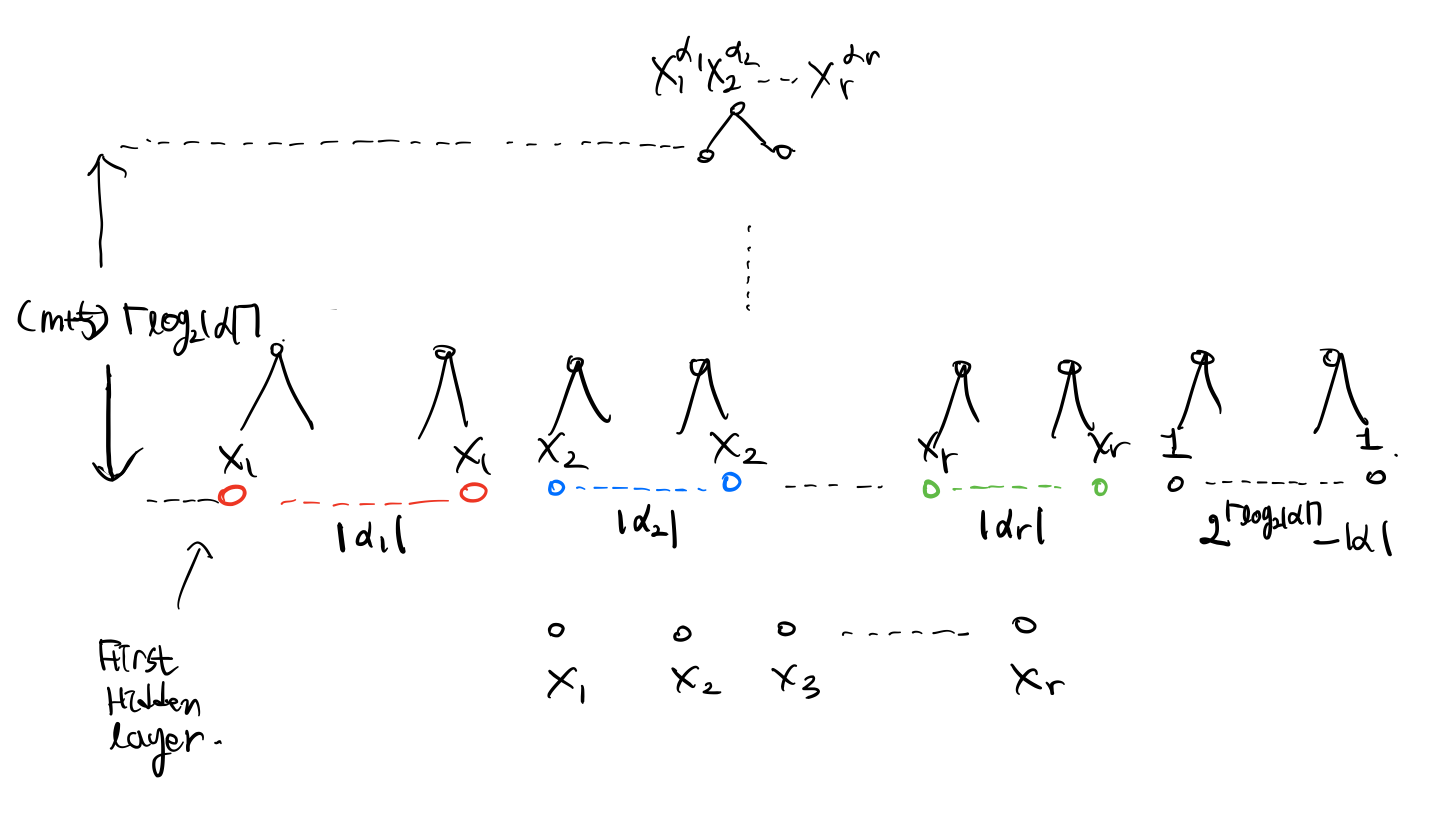
\includegraphics[width=0.8\textwidth]{LemmaA4.png}
        \label{fig:figure4}
    \end{figure}
\end{frame}

\subsection{Realization of $Hat^{r}(x_{1},\dots,x_{r})$}
\begin{frame}{Realization of $Hat^{r}(x_{1},\dots,x_{r})$}
\begin{tcolorbox}
    \textbf{(Lemma B.2.)}
    For any positive integer $M$ and $m$, there exists a network 
    \begin{align*}
        Hat^{r} \in \mathcal{F}&(2+(m+5) \ceil{\log_{2}r},\\
            &(r,6r(M+1)^{r},\dots,6r(M+1)^{r},(M+1)^{r}),s,1)
    \end{align*}
    with $s\leq 49r^{2}(M+1)^{r}(1+(m+5)\ceil{\log_{2}r})$ such that $Hat^{r}\in[0,1]^{(M+1)^{r}}$ and for any $\textbf{x}=(x_{1},x_{2},\dots,x_{r})\in[0,1]^{r}$,
    \begin{equation*}
        \left| Hat^{r}(x)-\bigg(\prod_{j=1}^{r}\bigg(\frac{1}{M}-|x_j - x_j^{\ell}|\bigg)_{+} \bigg)_{x_{\ell}\in D(M)} \right|_{\infty} \leq r^{2}2^{-m}.
    \end{equation*}
    For any $x_{\ell} \in D(M)$, the support of the function $x\rightarrow{(Hat^{r}(x))_{x_\ell}}$ is moreover contained in the support of the function $x\rightarrow{\prod_{j=1}^{r}(1/M - |x_{j}-x_{j}^{\ell}|)_{+}}$.
\end{tcolorbox}

\end{frame}

\begin{frame}{Realization of $Hat^{r}(x_{1},\dots,x_{r})$}
\begin{enumerate}
    \item Main goal of this Lemma is to construct a neural network which can approximate $\prod_{j=1}^{r}(1/M - |x_{j}-x_{j}^{\ell}|)_{+}$ for all the points in the grid (i.e. $\forall x_{\ell}\in D(M)$) with high accuracy.
    
    \item First, for each coordinate of $x_{j}$, we need to build a network layer which computes $(1/M - |x_{j}-\ell/M|)_{+}$ for all $\ell\in\{0,\dots,M\}$.
    
    \item Second, choose one out of $M+1$ quantities for each coordinate index and apply $Mult_{m}^{r}$ operator for those $r$ chosen values. 
\end{enumerate}
    \begin{figure}[htbp]
        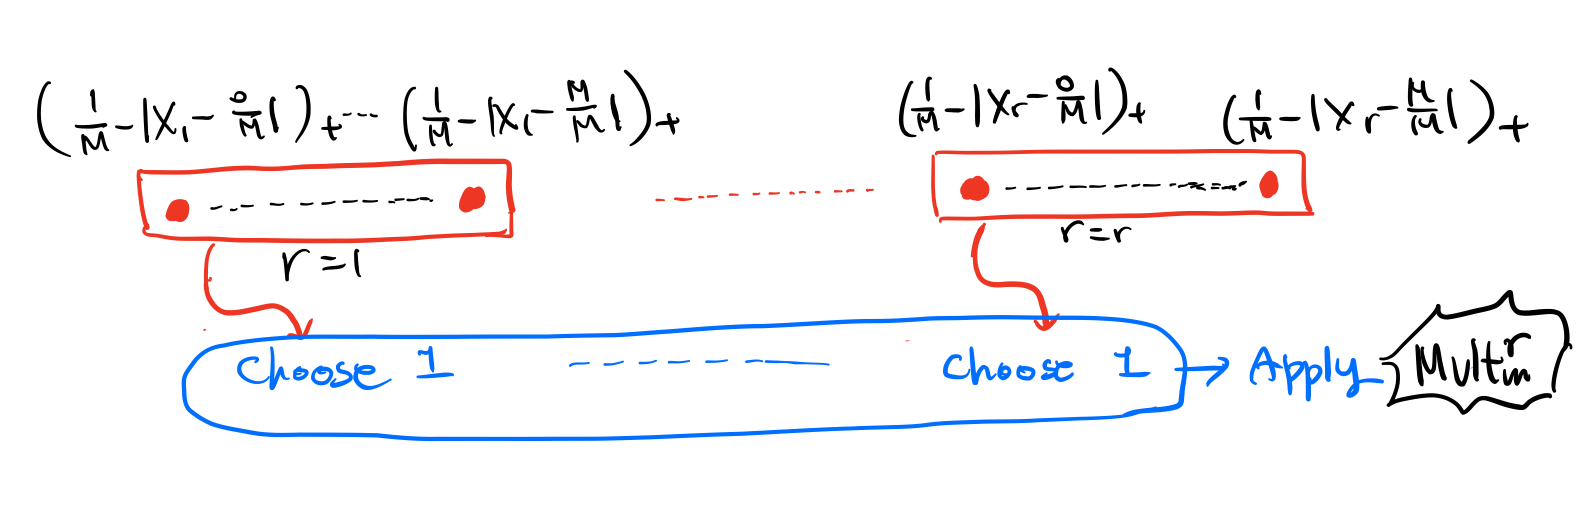
\includegraphics[width=1\textwidth]{LemmaB2.png}
        \label{fig:figure5}
    \end{figure}
\end{frame}

\begin{frame}{Realization of $Hat^{r}(x_{1},\dots,x_{r})$}
First two hidden layers of network $Hat^{r}$ can be constructed as follows:
Note that 
\begin{equation*}
    (1/M - |x_{j}-\ell/M|)_{+}=\big(1/M-(x_{j}-\ell/M)_{+}-(\ell/M-x_{j})_{+}\big)_{+}.
\end{equation*}

\begin{figure}[htbp]
    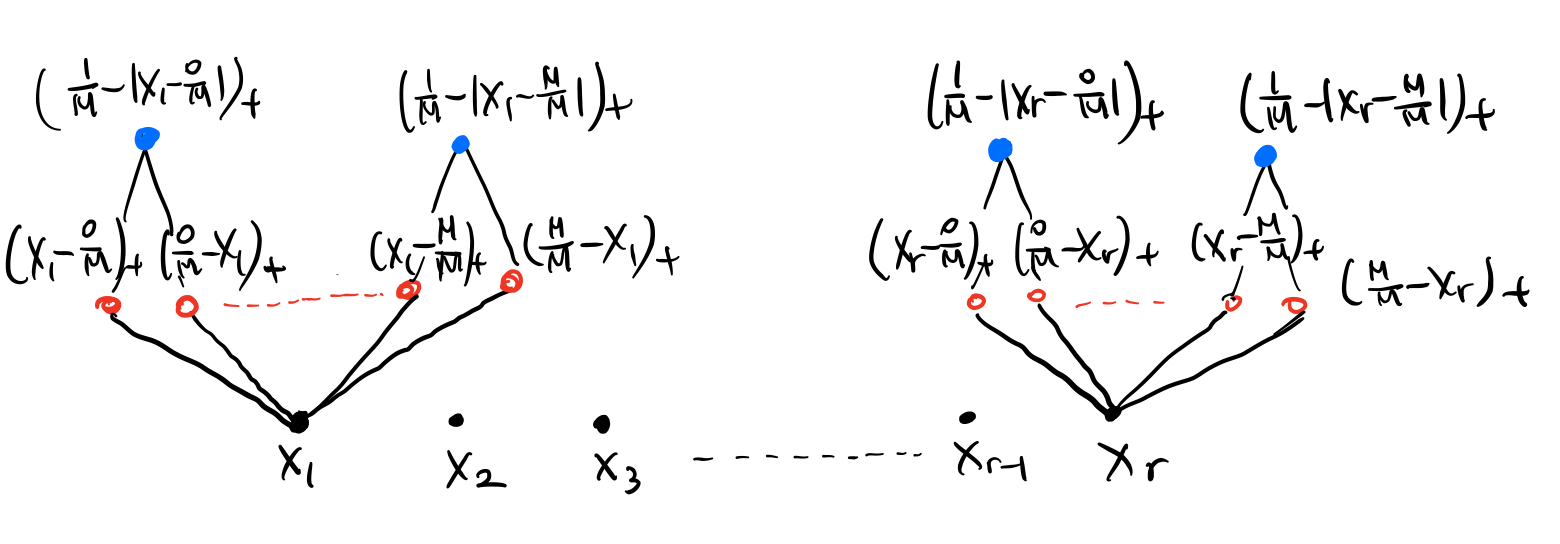
\includegraphics[width=1\textwidth]{LemmaB2_1.png}
    \label{fig:figure6}
\end{figure}

First hidden layer has $2r(M+1)$ nodes and $4r(M+1)$ non-zero weight parameters.
Second hiddn layer has $r(M+1)$ nodes and $3r(M+1)$ non-zero weight parameters.
    
\end{frame}


\begin{frame}{Realization of $Hat^{r}(x_{1},\dots,x_{r})$}

\begin{enumerate}
    \item It remains to apply $Mul_m^{r}$ operator to $r$ chosen values in second hidden layer of $Hat^{r}$.
    
    \item As there are $(M+1)^{r}$ of these networks, $Mul_m^{r}$, this requires $6r(M+1)^{r}$ units in each hidden layer and $42r^{2}(M+1)^{r}\big((m+5)\ceil{\log_{2}r}+1\big)$ non-zero parameters for the multiplication. 
    
    \item Note that the total number of non-zero parameters of the network in $\mathcal{F}(L,(p_{1},\dots,p_{L}))$ can be bounded by $\sum_{\ell=0}^{L}p_{\ell}p_{\ell+1}+\sum_{\ell=1}^{L}p_{\ell}$.

    \item Then non-zero parameters of $Mult_m^{r}$ can be bounded as follows:
    \begin{align*}
        &6r^{2}+36r^{2}((m+5)\ceil{\log_{2}r}-1)+6r+6r((m+5)\ceil{\log_{2}r})\\
        &=36r^{2}(m+5)\ceil{\log_{2}r}-30r^{2}+6r+6r(m+5)\ceil{\log_{2}r}\\
        &\leq 42r^{2}\big((m+5)\ceil{\log_{2}r}+1\big).
    \end{align*}
\end{enumerate}
\end{frame}

\begin{frame}{Realization of $Hat^{r}(x_{1},\dots,x_{r})$}
 \begin{enumerate}
     \item  Combining all the information elaborated above, we can finally construct a network which can approximate $\prod_{j=1}^{r}(1/M - |x_{j}-x_{j}^{\ell}|)_{+}$ for all $x_{\ell}\in D(M)$, whose network architecture is as follows:
    \begin{align*}
        Hat^{r} \in \mathcal{F}&(2+(m+5) \ceil{\log_{2}r},\\
            &(r,6r(M+1)^{r},\dots,6r(M+1)^{r},(M+1)^{r}),s,1)
    \end{align*}
    \item The number of non-zero parameters $s$ can be controlled trivially as follows : 
    \begin{align*}
        s&\leq 42r^{2}(M+1)^{r}\big((m+5)\ceil{\log_{2}r}+1\big) + 7r(M+1)\\
        &\leq 49r^{2}(M+1)^{r}\big((m+5)\ceil{\log_{2}r}+1\big)
    \end{align*}
\end{enumerate}
\end{frame}

\section{Third Step.}
\subsection{Key Idea for the Third Step}
\begin{frame}{Key Idea for the Third Step}
    Now we are ready to construct a neural network, $\Tilde{f}$, which can approximate Local Taylor Approximated $f(x)$ defined as:
    \begin{equation*}
        \sum_{x_{\ell}\in D(M)}P_{x_{\ell}}^{\beta}f(x)\prod_{j=1}^{r}\bigg( 1- M|x_{j}-x_{j}^{\ell}| \bigg)_{+} 
    \end{equation*}
    For all points in the grid $x_{\ell}\in D(M)$, we know how to construct neural networks which approximate : 
    \begin{equation*}
        P_{x_{\ell}}^{\beta}f(x) \quad \text{and} \quad \prod_{j=1}^{r}\big( 1/M - |x_{j}-x_{j}^{\ell}| \big)_{+},
    \end{equation*}
    through $Mon_{m,\gamma}^{r}$ and $Hat^{r}$, respectively.
    However, in order to realize an inner-product of outputs from these two networks through a fully-connected neural network with ReLU activation function, we need one more trick.
\end{frame}

\begin{frame}{Key Idea for the Third Step}
    Imagine we have a neural network, $\Phi_{1}\in [-1,1]$, which can approximate $\sin(x)$ function and  another neural network, $\Phi_{2}\in [-1,1]$, which approximates $\cos(x)$ function. 
    We want to have a neural network approximating $\sin(x)+\cos(x)$ through $\Phi_{1}$ and $\Phi_{2}$. For the construction of network, we apply ReLU activation function. 
    We need to construct a network in a following way : 
    \begin{figure}[htbp]
        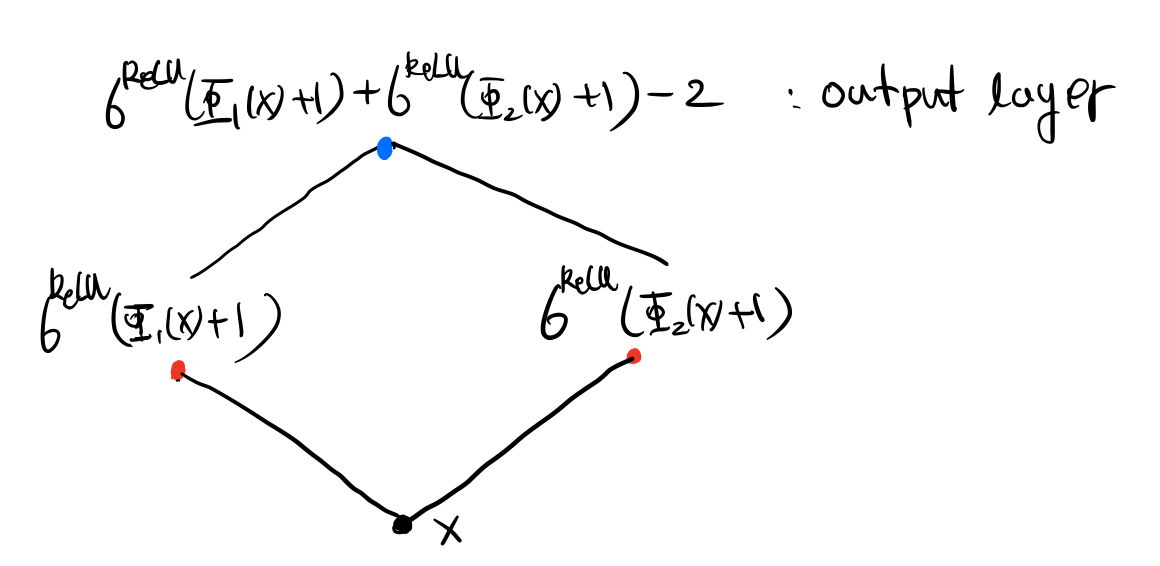
\includegraphics[width=0.8\textwidth]{Shift_Scale.png}
    \label{fig:figure7}
\end{figure}
\end{frame}

\subsection{Bound on $P^{\beta}_{x_{\ell}}f(x)$}
\begin{frame}{Bound on $P^{\beta}_{x_{\ell}}f(x)$}
    By using the aforementioned idea, we need to scale and shift $P^{\beta}_{x_{\ell}}f(x)$ so that the modified value is in $[0,1]$. In order to do this, we first need to obtain the maximum of $P^{\beta}_{x_{\ell}}f(x)$.
    Recall $P^{\beta}_{x_{\ell}}f(x)$ is defined as: 
     \begin{equation*}
        P_{x_{\ell}}^{\beta}f(x):=\sum_{\alpha:|\alpha|\leq n}(\partial^{\alpha}f)(x_{\ell})\frac{(x-x_{\ell})^{\alpha}}{\alpha!}
    \end{equation*}
    By $r$-dimensional binomial theorem, we can rewrite $(x-x_{\ell})^{\alpha}$ as 
    \begin{equation*}
        (x-x_{\ell})^{\alpha}=\sum_{\gamma \leq \alpha} {\alpha \choose \gamma} (-x_{\ell})^{\alpha-\gamma}x^{\gamma}, \quad
        \forall x \in [0,1]^{r}, \alpha \in \mathbb{N}_{0}^{r}.  
    \end{equation*}
    Here for vectors $\gamma,\alpha \in \mathbb{N}_{0}^{r}$, $\gamma \leq \alpha$ means that 
    \begin{equation*}
        \gamma_{1}\leq\alpha_{1},\dots,\gamma_{r}\leq\alpha_{r}.
    \end{equation*}
\end{frame}

\begin{frame}{Bound on $P^{\beta}_{x_{\ell}}f(x)$}
    Then we can write $P^{\beta}_{x_{\ell}}f(x)$ as follows:
    \begin{align*}
        P_{x_{\ell}}^{\beta}f(x)&=\sum_{\alpha:|\alpha|\leq n}\frac{(\partial^{\alpha}f)(x_{\ell})}{\alpha!}
        \sum_{\gamma \leq \alpha} {\alpha \choose \gamma} (-x_{\ell})^{\alpha-\gamma}x^{\gamma}\\
        &=\sum_{\gamma:|\gamma|\leq n}
        \underbrace{\Bigg[\sum_{\gamma \leq \alpha \& |\alpha| \leq n} \frac{(\partial^{\alpha}f)(x_{\ell})}{\alpha!}{\alpha \choose \gamma} (-x_{\ell})^{\alpha-\gamma}\Bigg]}_{:=C_{\gamma}}x^{\gamma}.
    \end{align*}
    
    The absolute value of $C_{\gamma}$ can be controlled by using facts $x_{\ell}\in[0,1]^{r}$, $f\in\mathcal{C}_{r}^{\beta}([0,1]^{r},K)$ and $(\alpha-\gamma)!\geq 1$:
    For fixed $\gamma\in \mathbb{N}_{0}^{r}$
    \begin{align*}
        \left|C_{\gamma}\right| \leq \sum_{\gamma \leq \alpha \& |\alpha| \leq n} \frac{|(\partial^{\alpha}f)(x_{\ell})|}{(\alpha-\gamma)!\gamma!}|(-x_{\ell})^{\alpha-\gamma}|
        \leq \frac{K}{\gamma!}.
    \end{align*}
    Here, we omit the dependency of $x_{\ell}$ when writing $C_{\gamma}$ for simplicity.
\end{frame}

\begin{frame}{Bound on $P^{\beta}_{x_{\ell}}f(x)$}
    Finally, we can bound $P^{\beta}_{x_{\ell}}f(x),\forall x\in[0,1]^{r}$ as follows:
    \begin{align*}
        P_{x_{\ell}}^{\beta}f(x)&=\sum_{\gamma:|\gamma|\leq n} C_{\gamma}x^{\gamma}
        \leq \sum_{\gamma:|\gamma|\leq n} |C_{\gamma}| \\
        &\leq \sum_{\gamma \geq 0} |C_{\gamma}| \leq \sum_{\gamma \geq 0} \frac{K}{\gamma!} \\
        &= K \prod_{j=1}^{r} \sum_{\gamma_{j} \geq 0} \frac{1}{\gamma_{j}!}=Ke^{r}.
    \end{align*}
\end{frame}


\subsection{Third Step: Substep $1$.}
\begin{frame}{Third Step: Substep $\circled{1}$.}
Let $B=\ceil{2Ke^{r}}$. Then we are ready to construct a network, $Q_{1}$, which can approximate $\frac{P^{\beta}_{x_{\ell}}f(x)}{B}+\frac{1}{2}\in[0,1]^{(M+1)^{r}}$.
We can simply add one hidden layer to the network $Mon_{m,\beta}^{r}$ as follows : 

\begin{figure}[htbp]
    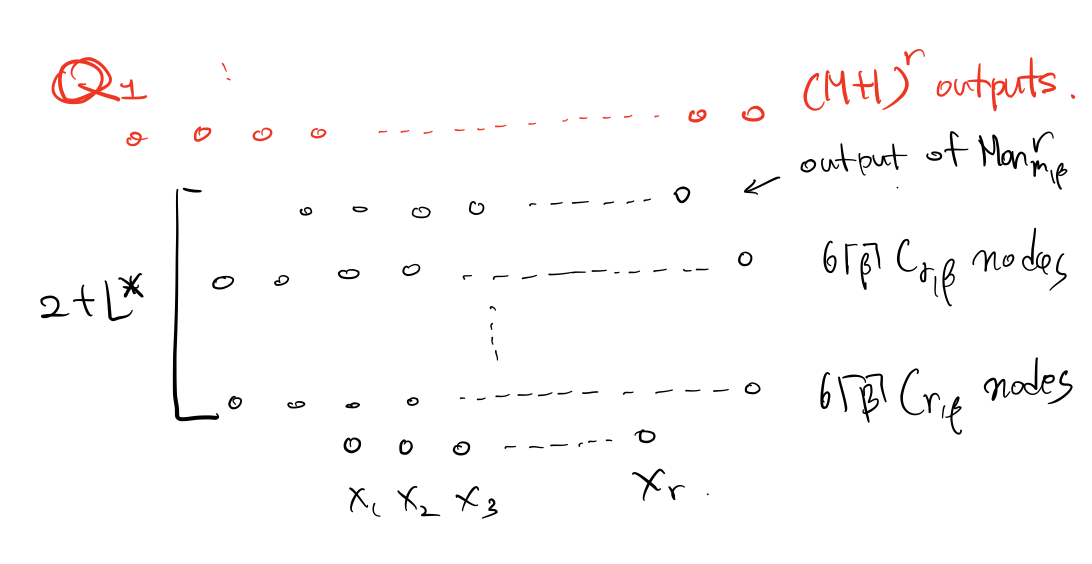
\includegraphics[width=0.8\textwidth]{Substep1.png}
    \label{fig:figure8}
\end{figure}
    
Note that all the absolute values of weight and bias parameters used for output layer are bounded by $1$, since $\frac{1}{B}|C_{\gamma,x_{\ell}}|\leq 1$ for all $\gamma:|\gamma|\leq n$, $x_{\ell}\in D(M)$.
We use $L^*:=(m+5)\ceil{\log_{2}(\beta\vee r)}$.
\end{frame}

\begin{frame}{Third Step: Substep $\circled{1}$.}
Note that $\frac{1}{2}$ can be added by putting $\frac{1}{B}C_{\gamma,x_{\ell}}+\frac{1}{2}$ weight on monomial $x^{0}=1$ for each $\gamma:|\gamma|\leq n$ and $x_{\ell}\in D(M)$.
\begin{figure}[htbp]
    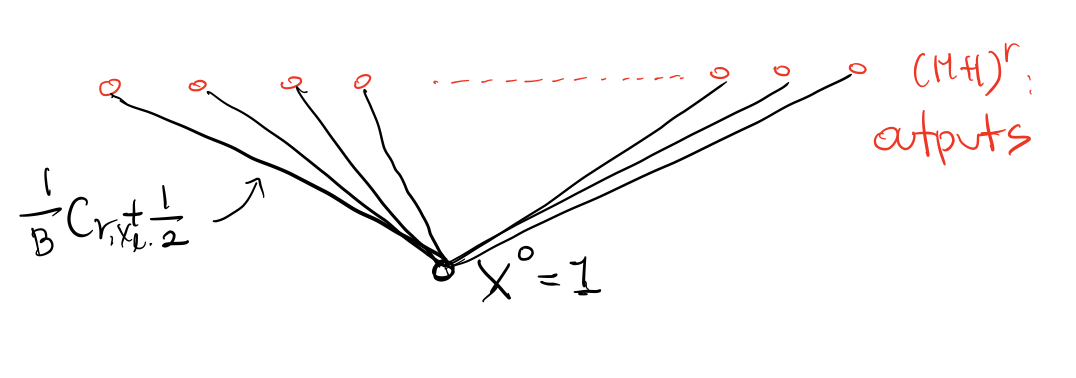
\includegraphics[width=0.8\textwidth]{one-half.png}
    \label{fig:figure9}
\end{figure}

Through these constructions, it is obvious that $Q_{1}$ has a following network structure:
\begin{equation*}
    Q_{1}\in \mathcal{F}\big(2+L^*,
            (r,6\ceil{\beta}C_{r,\beta},\dots,6\ceil{\beta}C_{r,\beta},C_{r,\beta},(M+1)^{r})\big),
\end{equation*}
such that $Q_{1}\in[0,1]^{(M+1)^{r}}$.
\end{frame}

\begin{frame}{Third Step: Substep $\circled{1}$.}
The approximation error in a $L^{\infty}$ sense of the network $Q_{1}$ for any $x\in[0,1]^{r}$ can be calculated trivially as : For any integer $m\geq 1$,
\begin{align*}
\left|Q_{1}(x)-\bigg( \frac{P^{\beta}_{x_{\ell}}f(x)}{B} + \frac{1}{2} \bigg)_{x_{\ell}\in D(M)} \right|_{\infty}
&\leq \frac{1}{B}\sum_{\gamma:|\gamma|\leq n}|C_{\gamma}|\beta^{2}2^{-m}\\
&\leq \frac{Ke^{r}}{B}\beta^{2}2^{-m}\leq \beta^{2}2^{-m}. 
\end{align*}
Total number of non-zero parameters can be bounded as :
\begin{align*}
6r(\beta+1)C_{r,\beta}+42(\beta+1)^{2}C_{r,\beta}^{2}(1+L^*)+C_{r,\beta}(M+1)^{r}.
\end{align*}
\end{frame}

\subsection{Third Step: Substep $2$.}
\begin{frame}{Third Step: Substep $\circled{2}$.}
Consider now a parallel network $(Q_{1},Hat^{r})$:
\begin{enumerate}
    \item Observe that $C_{r,\beta} \leq (\beta+1)^{r} \leq N$ by the definition of $C_{r,\beta}$ and the assumptions on $N$ in the statement of Theorem 5. 
    \item The parallelized network $(Q_{1},Hat^{r})$ has a following architecture :
    \begin{align*}
        (Q_{1},Hat^{r}) \in \mathcal{F}&(2+(m+5) \ceil{\log_{2}(r \vee \beta)},\\
            &(r,6(r+\ceil{\beta})N,\dots,6(r+\ceil{\beta})N,2(M+1)^{r}))
    \end{align*}
    \item Note that all network parameters are bounded by $1$.
\end{enumerate}

\end{frame}

\begin{frame}{Third Step: Substep $\circled{2}$.}
The total number of network parameter of $(Q_{1}, Hat^{r})$ can be bounded as follows:
We set $M$ to be the largest integer such that $(M+1)^{r} \leq N$.
    \begin{align*}
        &6r(\beta+1)C_{r,\beta} +42(\beta+1)^{2}C_{r,\beta}^{2}(L^*+1) + C_{r,\beta}(M+1)^{r} + 49r^{2}(M+1)^{r}(L^*+1) \\
        &\leq 6r(\beta+1)C_{r,\beta}N(1+L^*) + 42(\beta+1)^{2}C_{r,\beta}N(1+L^*)  + C_{r,\beta}N(1+L^*) + 49r^{2}C_{r,\beta}N(1+L^*)\\
        &\leq 49(\beta^{2}+2\beta+1+r\beta+r+r^{2}+1)C_{r,\beta}N(1+L^*)\\
        &\leq 49(\beta+r+1)^{2}C_{r,\beta}N(1+L^*)\\
        &\leq 49(\beta+r+1)^{2+r}N(1+L^*)\\
        &\leq 98(\beta+r+1)^{3+r}N(m+5)
    \end{align*}
where in the last inequality, we use the fact:
\begin{align*}
    1+(m+5)\ceil{\log_{2}(\beta \vee r)} 
    &\leq (m+5) \big( 1+\ceil{\log_{2}(\beta \vee r)}\big)\\
    &\leq 2(m+5)(\beta \vee r)\\
    &\leq 2(m+5)(\beta + r + 1).
\end{align*}
\end{frame}

\subsection{Third Step: Substep $3$.}
\begin{frame}{Third Step: Substep $\circled{3}$.}
\begin{enumerate}
    \item Next, we pair the $x_{\ell}$th entry of $Q_{1}$ and $Hat^{r}$ and apply to each of the $(M+1)^{r}$ pairs the $Mult_m$ network described in $Lemma.A.2.$
    \item In the last layer, we add up all entries.
    \item Finally, we have a network $Q_{2}$ which can approximate
    \begin{equation*}
        \sum_{x_{\ell}\in D(M)}\bigg( \frac{P_{x_{\ell}}^{\beta}f(x)}{B}+\frac{1}{2}\bigg)\prod_{j=1}^{r}\bigg( \frac{1}{M} - |x_{j}-x_{j}^{\ell}| \bigg)_{+}.
    \end{equation*}
    \item The network's architecture is as follows:
    \begin{align*}
        Q_{2} \in \mathcal{F}&(3+(m+5) \big( 1 + \ceil{\log_{2}(r \vee \beta)} \big),\\
            &(r,6(r+\ceil{\beta})N,\dots,6(r+\ceil{\beta})N,1)).
    \end{align*}
\end{enumerate}
\end{frame}

\begin{frame}{Third Step: Substep $\circled{3}$.}
    Note that the required number of parameters for $Mult_{m}$ is at most :
    \begin{align*}
        6+12+36(m+3)+6(m+4) \leq 42(m+5)
    \end{align*}
    We need $(M+1)^{r}$ $Mult_{m}$s serially and $(M+1)^{r}$ parameters for adding up entries in the last hidden layer.
    This means that at least 
    \begin{align*}
         42(m+5)(M+1)^{r}+(M+1)^{r} \leq 43(m+5)N
    \end{align*}
    non-zero parameters are required for the steps $1.$ and $2.$ in the previous slide.
    By combining the bound we obtained for the number of non-zero parameters for $(Q_{1},Hat^{r})$ network, the $s$ for $Q_2$ is bounded by :
    \begin{equation*}
        141(r+\beta+1)^{3+r}N(m+5).
    \end{equation*}
\end{frame}
    
\begin{frame}{Third Step: Substep $\circled{3}$.}
By triangular inequality, we can get the approximation error bound for $Q_2$:
\begin{align*}
    &\left| Q_{2} - \sum_{x_{\ell}\in D(M)}\bigg( \frac{P_{x_{\ell}}^{\beta}f(x)}{B}+\frac{1}{2}\bigg)\prod_{j=1}^{r}\bigg( \frac{1}{M} - |x_{j}-x_{j}^{\ell}| \bigg)_{+}  \right| \\
    &\leq \sum_{x_{\ell}\in D(M): \|x-x_{\ell}\|_{\infty}\leq 1/M} (1+r^{2}+\beta^{2}) 2^{-m} \\
    &\leq (1+r^{2}+\beta^{2}) 2^{r-m}.
\end{align*}
In the last inequality, we use the fact for any $x\in[0,1]^{r}$, there are $2^{r}$ points in the grid $D(M)$ whose $L^{\infty}$ distance between an input data $x$ is within $1/M$.
\end{frame}

\subsection{Third Step: Substep $4$.}
\begin{frame}{Third Step: Substep $\circled{4}$.}
Finally, we need a network operator which can perform re-scaling and re-shifting as follows:

\begin{align*}
    \sum_{x_{\ell}\in D(M)}\bigg( \frac{P_{x_{\ell}}^{\beta}f(x)}{B}&+\frac{1}{2}\bigg)\prod_{j=1}^{r}\bigg( \frac{1}{M} - |x_{j}-x_{j}^{\ell}| \bigg)_{+} \\
    &\rightarrow{\sum_{x_{\ell}\in D(M)} P_{x_{\ell}}^{\beta}f(x)\prod_{j=1}^{r}\bigg( 1 - M|x_{j}-x_{j}^{\ell}| \bigg)_{+}}
\end{align*}

Note that
\begin{align*}
    \sum_{x_{\ell}\in D(M)}\bigg( &\frac{P_{x_{\ell}}^{\beta}f(x)}{B}+\frac{1}{2}\bigg)\prod_{j=1}^{r}\bigg( \frac{1}{M} - |x_{j}-x_{j}^{\ell}| \bigg)_{+} \\
    &= \underbrace{\frac{1}{BM^{r}}\sum_{x_{\ell}\in D(M)} P_{x_{\ell}}^{\beta}f(x)\prod_{j=1}^{r}\bigg( 1 - M|x_{j}-x_{j}^{\ell}| \bigg)_{+}+\frac{1}{2M^{r}}}_{:=a}.
\end{align*}
\end{frame}

\begin{frame}{Third Step: Substep $\circled{4}$.}
We need a network operator with ReLU activation function computing $a\rightarrow{BM^{r}(a-1/2M^{r})}$.
\begin{enumerate}
    \item The network $x\rightarrow{BM^{r}x}$ is in the class $\mathcal{F}(3,(1,M^{r},1,B,1))$ with shift vectors $v_{j}$ are all equal to zero and weight matrices $W_{j}$ having all entries equal to one.
    \begin{figure}[htbp] 
        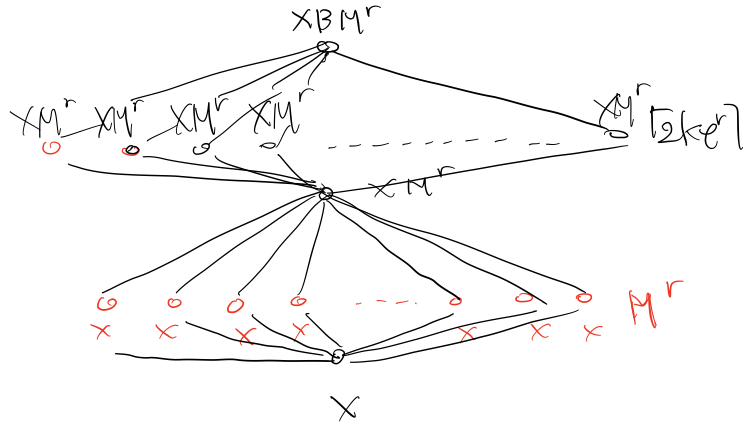
\includegraphics[width=0.5\textwidth]{final_step.png}
    \end{figure}
    \item Network $a\rightarrow{BM^{r}(a-1/2M^{r})}$ computes in the first hidden layer $(a-1/2M^{r})_{+}$ and $(1/2M^{r}-a)_{+}$ and then applies the network $x\rightarrow{BM^{r}x}$ to both units. In the output layer the second value is subtracted from the first one. 
\end{enumerate}
\end{frame}

\begin{frame}{Third Step: Substep $\circled{4}$.}
It is trivial to check network $a\rightarrow{BM^{r}(a-1/2M^{r})}$ has at most $12N+6$ non-zero parameters.
\begin{enumerate}
    \item For the network $x\rightarrow{BM^{r}x}$, we need $2M^{r}+2\ceil{2Ke^{r}}$ parameters. Because of the assumption $N\geq (K+1)e^{r}$, at most $6N$ parameters are required.
    \item We need two $x\rightarrow{BM^{r}x}$ networks and extra $6$ parameters for the network  $a\rightarrow{BM^{r}(a-1/2M^{r})}$.
\end{enumerate}
\end{frame}

\begin{frame}{Third Step: Substep $\circled{4}$.}
Apply the network $a\rightarrow{BM^{r}(a-1/2M^{r})}$ to the output of $Q_{2}$, then there exists a network $Q_{3}$ in 
    \begin{align*}
        Q_{3} \in \mathcal{F}&(8+(m+5) \big( 1 + \ceil{\log_{2}(r \vee \beta)} \big),\\
            &(r,6(r+\ceil{\beta})N,\dots,6(r+\ceil{\beta})N,1)),
    \end{align*}
such that, for all $x\in[0,1]^{r}$,
\begin{align*}
    &\left| Q_{3} -\sum_{x_{\ell}\in D(M)} P_{x_{\ell}}^{\beta}f(x)\prod_{j=1}^{r}\bigg( 1 - M|x_{j}-x_{j}^{\ell}| \bigg)_{+} \right| \\
    &\leq \ceil{2Ke^{r}}M^{r}(1+r^{2}+\beta^{2}) 2^{r-m} \\
    &\leq (2K+1)(2e)^{r}M^{r}(1+r^{2}+\beta^{2}) 2^{-m} \\
    &\leq (2K+1)(1+r^{2}+\beta^{2}) 6^{r} N 2^{-m}.
\end{align*}

\end{frame}

\begin{frame}{Third Step: Substep $\circled{4}$.}
    The number of non-zero parameters of $Q_{3}$ is bounded by
    \begin{equation*}
        141(r+\beta+1)^{3+r}N(m+5) + (12N+6)
        \leq 141(r+\beta+1)^{3+r}N(m+6).
    \end{equation*}

    We are ready to obtain an approximation error bound : 
    \begin{align*}
        \left\| \Tilde{f} - f \right\|_{L^\infty[0,1]^{r}}
        &\leq \left\| P^{\beta}f(X) - f(X) \right\|_{L^\infty[0,1]^{r}} +
        \left\| \Tilde{f} - P^{\beta}f(X) \right\|_{L^\infty[0,1]^{r}} \\
        &\leq KM^{-\beta} + (2K+1)(1+r^{2}+\beta^{2}) 6^{r} N 2^{-m} \\
        &\leq 3^\beta N^{-\frac{\beta}{r}} + (2K+1)(1+r^{2}+\beta^{2}) 6^{r} N 2^{-m}.
    \end{align*}
    where in the last inequality, we use 
    \begin{equation*}
        (M+1)^{r}\leq N \leq (M+2)^{r} \leq (3M)^{r}.
    \end{equation*}
    We finally conclude the proof.
\end{frame}

% Uncomment these lines for an automatically generated outline.
%\begin{frame}{Outline}
%  \tableofcontents
%\end{frame}

\end{document}